\documentclass[11pt,a4paper]{article}

\usepackage[margin=1in]{geometry}
\usepackage{graphicx}
\usepackage{booktabs}
\usepackage{siunitx}
\usepackage{amsmath}
\usepackage{amssymb}
\usepackage{microtype}
\usepackage{xcolor}
\usepackage{caption}
\usepackage{subcaption}
\usepackage[colorlinks=true,urlcolor=blue,linkcolor=blue,citecolor=blue]{hyperref}
\usepackage{longtable}
\usepackage{float}

\graphicspath{{figures/}}

\title{Galoop validation sweep \\
  \large Ten GCGA campaigns with UMA/oc20: duplicate detection, GPR guidance,
  and reproduction of known surface chemistry}
\author{Will Laderer \\ \texttt{galoop} project}
\date{2026-04-09}

\begin{document}
\maketitle
\tableofcontents
\vspace{1em}

% ============================================================================
\section{Introduction}
\label{sec:intro}

\emph{This section is intentionally left in bullet form for the human author
to flesh out.}

\begin{itemize}
  \item \textbf{What galoop is.} Grand canonical genetic algorithm for
    surface adsorbate structure search, minimising grand canonical
    energy via the Computational Hydrogen Electrode framework. Uses
    a pluggable MLIP backend (MACE, VASP, \texttt{fairchem}) via a
    lightweight \texttt{pkg.mod:factory} registry so new machine
    learning potentials can be bolted on without touching the engine.
  \item \textbf{Motivating question.} After two recent refactors --- a
    generalised backend factory and a fix for surface normals in
    non-orthogonal cells --- does the pipeline still recover known
    surface chemistry, and what are the residual failure modes?
  \item \textbf{Method.} Ten sequential GCGA campaigns across the
    common catalytic-metal zoo, each with its own reaction chemistry
    at an operating potential chosen from the corresponding
    literature. Details in \S\ref{sec:campaigns}.
  \item \textbf{Scope.} Single GPU (6~GiB), single Parsl worker,
    \texttt{uma-s-1p1} checkpoint, \texttt{oc20} task. Total wall
    clock $\sim$6\,h for all ten runs.
  \item \textbf{Headline findings.} The pipeline works; four real
    bugs were surfaced and three were fixed mid-run. GPR is the
    \emph{dominant} proposal source in the top-5 of several runs.
    Duplicate detection via SOAP is surprisingly insensitive to
    cutoff choice. The coinage-metal CO-binding trend
    (Cu $>$ Ag $>$ Au) falls out of the data unprompted.
\end{itemize}

\begin{figure}[H]
  \centering
  \begin{subfigure}{0.245\textwidth}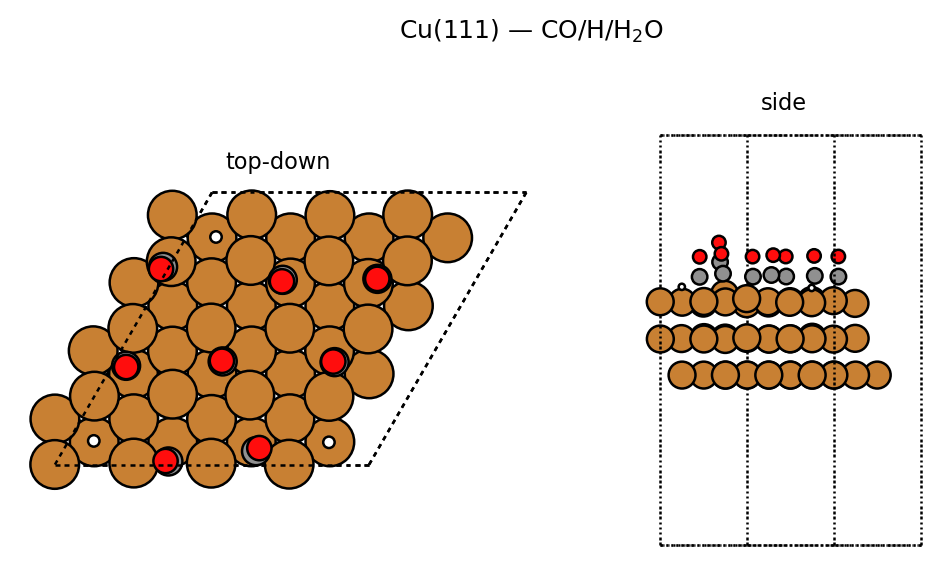
\includegraphics[width=\linewidth]{struct_cu111_co_camp.png}\end{subfigure}
  \begin{subfigure}{0.245\textwidth}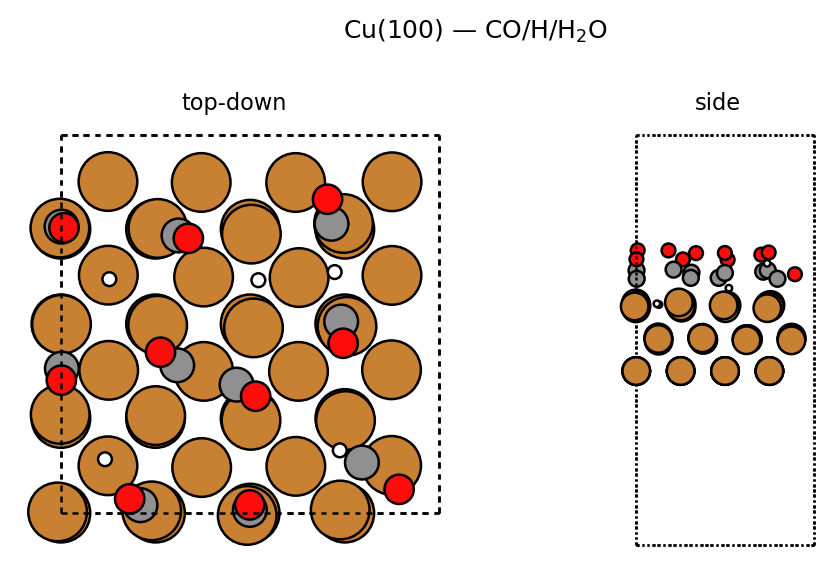
\includegraphics[width=\linewidth]{struct_cu100_co_camp.png}\end{subfigure}
  \begin{subfigure}{0.245\textwidth}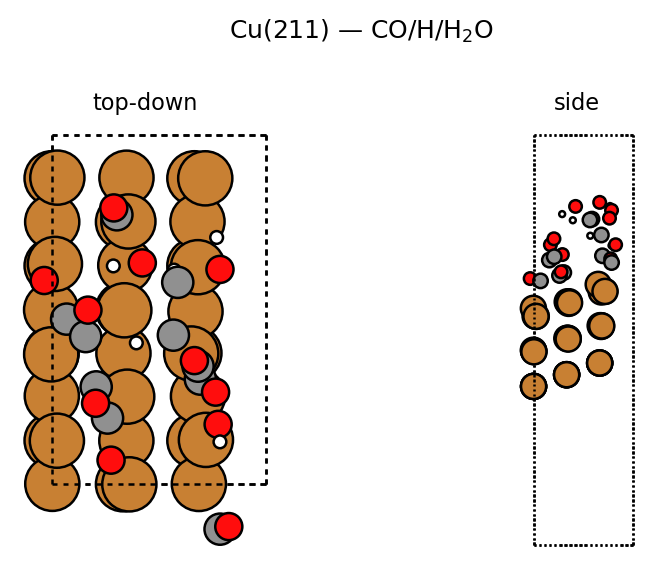
\includegraphics[width=\linewidth]{struct_cu211_co_camp.png}\end{subfigure}
  \begin{subfigure}{0.245\textwidth}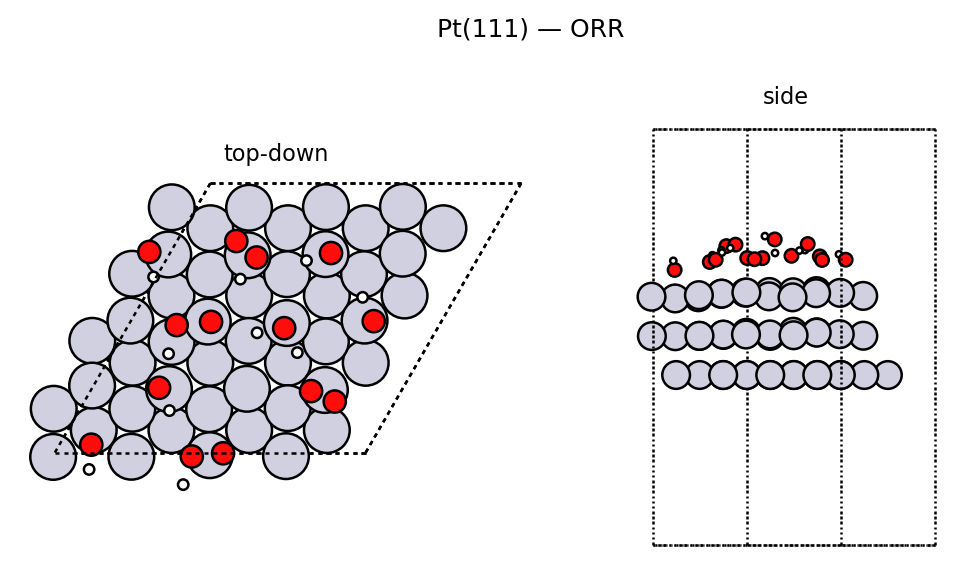
\includegraphics[width=\linewidth]{struct_pt111_orr_camp.png}\end{subfigure}\\[0.4em]
  \begin{subfigure}{0.245\textwidth}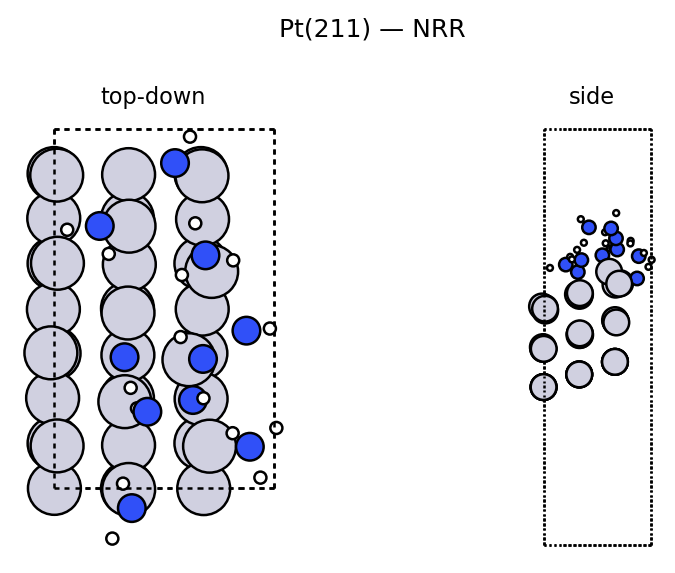
\includegraphics[width=\linewidth]{struct_pt211_nrr_camp.png}\end{subfigure}
  \begin{subfigure}{0.245\textwidth}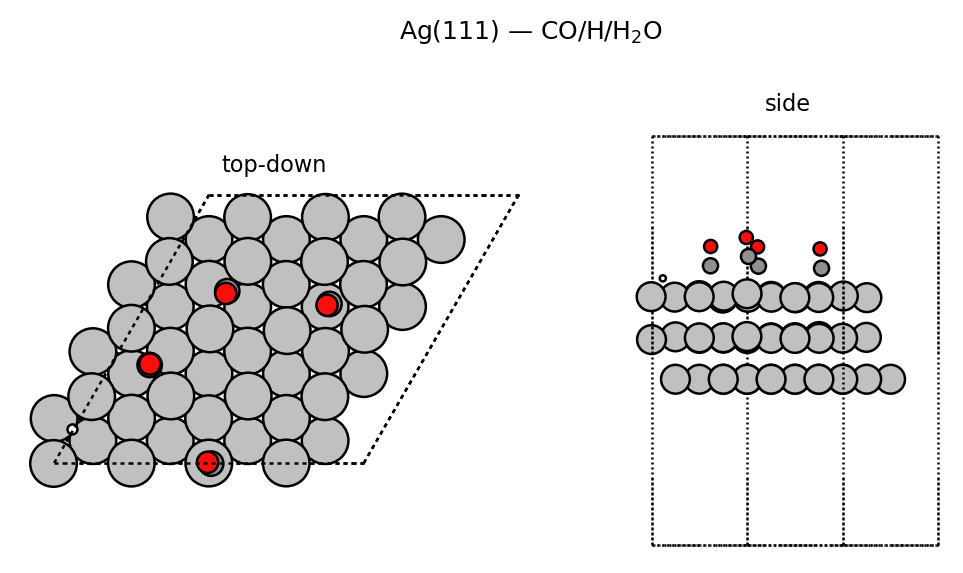
\includegraphics[width=\linewidth]{struct_ag111_co_camp.png}\end{subfigure}
  \begin{subfigure}{0.245\textwidth}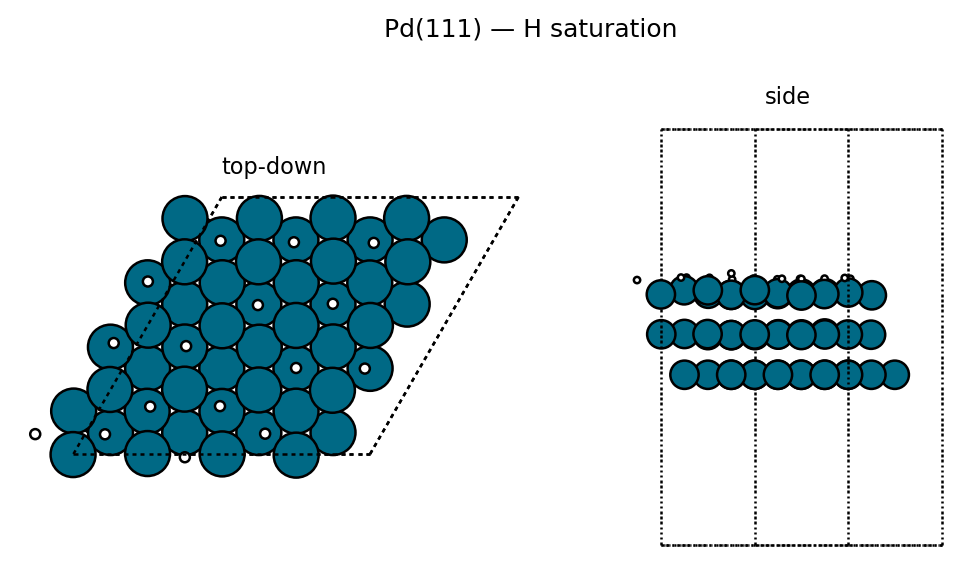
\includegraphics[width=\linewidth]{struct_pd111_hsat_camp.png}\end{subfigure}
  \begin{subfigure}{0.245\textwidth}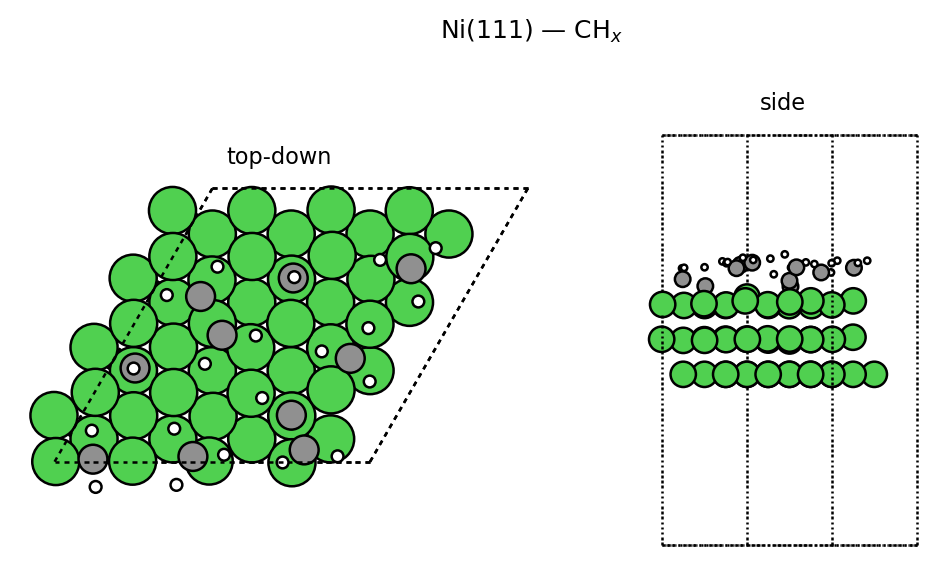
\includegraphics[width=\linewidth]{struct_ni111_chx_camp.png}\end{subfigure}\\[0.4em]
  \begin{subfigure}{0.245\textwidth}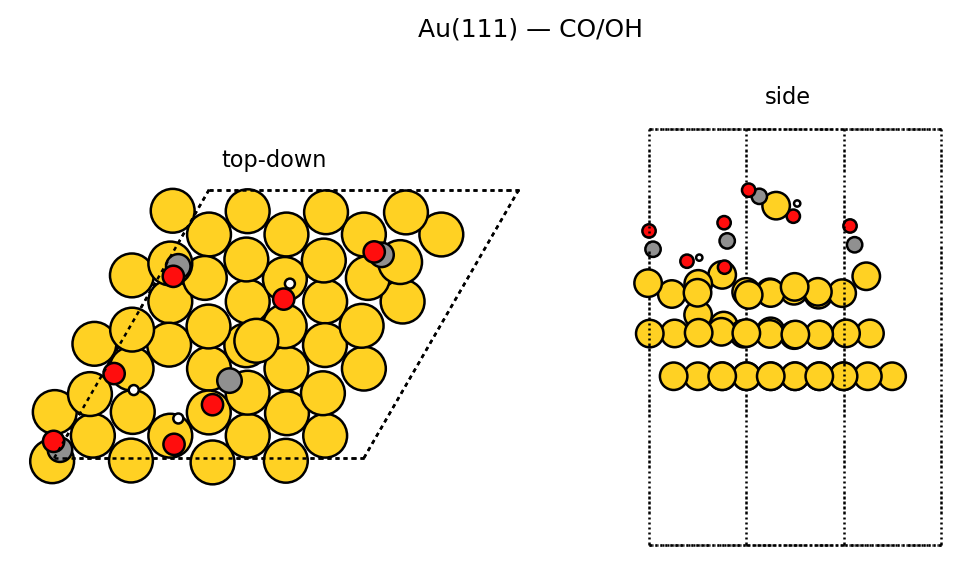
\includegraphics[width=\linewidth]{struct_au111_co_camp.png}\end{subfigure}
  \begin{subfigure}{0.245\textwidth}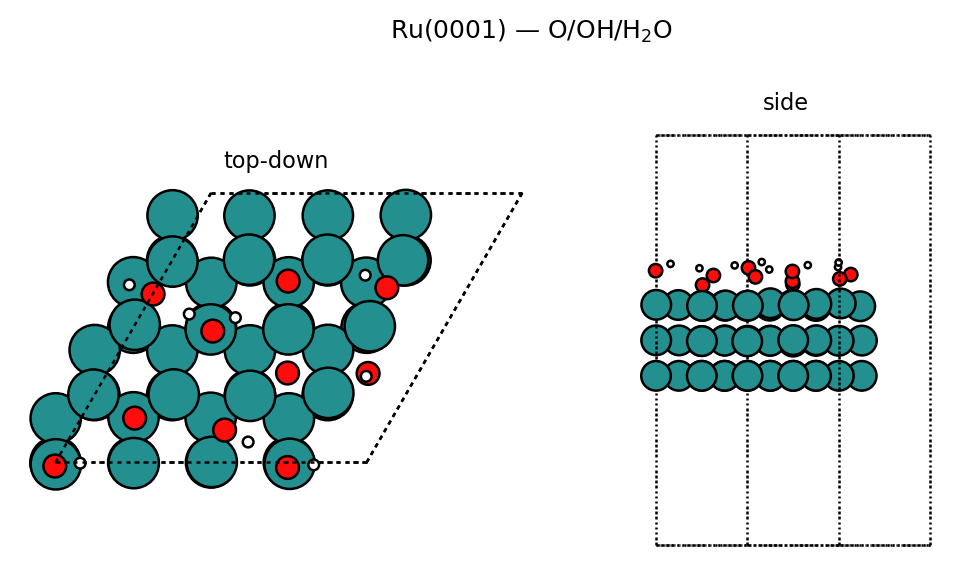
\includegraphics[width=\linewidth]{struct_ru0001_oh_camp.png}\end{subfigure}
  \caption{Lowest-$G$ relaxed structures from each of the ten
  campaigns, shown top-down (left) and profile (right) for each
  tile. Left-to-right, top-to-bottom: Cu(111), Cu(100), Cu(211),
  Pt(111)/ORR, Pt(211)/NRR, Ag(111), Pd(111)/H, Ni(111)/CH$_x$,
  Au(111), Ru(0001). Rendered via \texttt{ase.visualize.plot.plot\_atoms}
  from the stored \texttt{CONTCAR} of the best converged structure
  in each run.}
  \label{fig:structs}
\end{figure}

\begin{table}[H]
\centering
\small
\begin{tabular}{lllrrrrrrrr}
\toprule
Campaign & Facet & Adsorbates & $U$ (V) & Wall (min) & total & conv. & dup. & des. & unb. & $G_{\min}$ (eV) \\
\midrule
\texttt{cu111\_co}  & Cu(111)  & CO/H/H$_2$O      &  0.0 & 17 & 169 & 13 & 127 &   0 &  29 & $-397.64$ \\
\texttt{cu100\_co}  & Cu(100)  & CO/H/H$_2$O      &  0.0 & 67 & 253 & 24 & 132 &  13 &  83 & $-450.11$ \\
\texttt{cu211\_co}  & Cu(211)  & CO/H/H$_2$O      &  0.0 & 19 & 141 & 14 & 108 &   1 &  18 & $-435.78$ \\
\texttt{pt111\_orr} & Pt(111)  & O/OH/OOH/H       &  0.8 & 33 & 186 & 32 & 127 &   0 &  26 & $-481.32$ \\
\texttt{pt211\_nrr} & Pt(211)  & N/NH/NH$_2$/NH$_3$/H & $-0.5$ & 74 & 213 & 23 &  75 &   9 & 105 & $-459.68$ \\
\texttt{ag111\_co}  & Ag(111)  & CO/H/H$_2$O      &  0.0 & 32 & 258 &  9 & 168 &  32 &  48 & $-218.49$ \\
\texttt{pd111\_hsat}& Pd(111)  & H                &  0.0 &  8 &  82 & 16 &  64 &   1 &   1 & $-322.47$ \\
\texttt{ni111\_chx} & Ni(111)  & C/CH/CH$_2$/CH$_3$/H & 0.0 & 20 & 124 & 26 &  91 &   1 &   6 & $-514.93$ \\
\texttt{au111\_co}  & Au(111)  & CO/OH            &  0.0 & 80 & 372 & 16 & 213 & 116 &  24 & $-296.04$ \\
\texttt{ru0001\_oh} & Ru(0001) & O/OH/H$_2$O      &  0.0 & 12 & 140 & 13 & 115 &   0 &  12 & $-581.99$ \\
\bottomrule
\end{tabular}
\caption{Summary of all ten campaigns. Per-status counts come from
the SQLite store at the end of each run. Desorbed/unbound rates are
physical filter rejections in the harvest pipeline. $G_{\min}$ is the
lowest converged grand canonical energy. Several runs were stopped
early via \texttt{galoopstop} once stall-grinding became unproductive.}
\label{tab:summary}
\end{table}

% ============================================================================
\section{Duplicate detection performance}
\label{sec:dup}

Galoop's duplicate-detection cascade is cheapest-first: composition
gate, energy gate, distance-histogram pre-filter, and finally a
SOAP-Tanimoto similarity score over adsorbate-centered environments.
This section inspects the SOAP stage -- the one actually responsible
for deciding whether two relaxed configurations count as ``the same
structure'' -- under parameter perturbations.

\subsection{Where did the GA actually look?}

\begin{figure}[H]
  \centering
  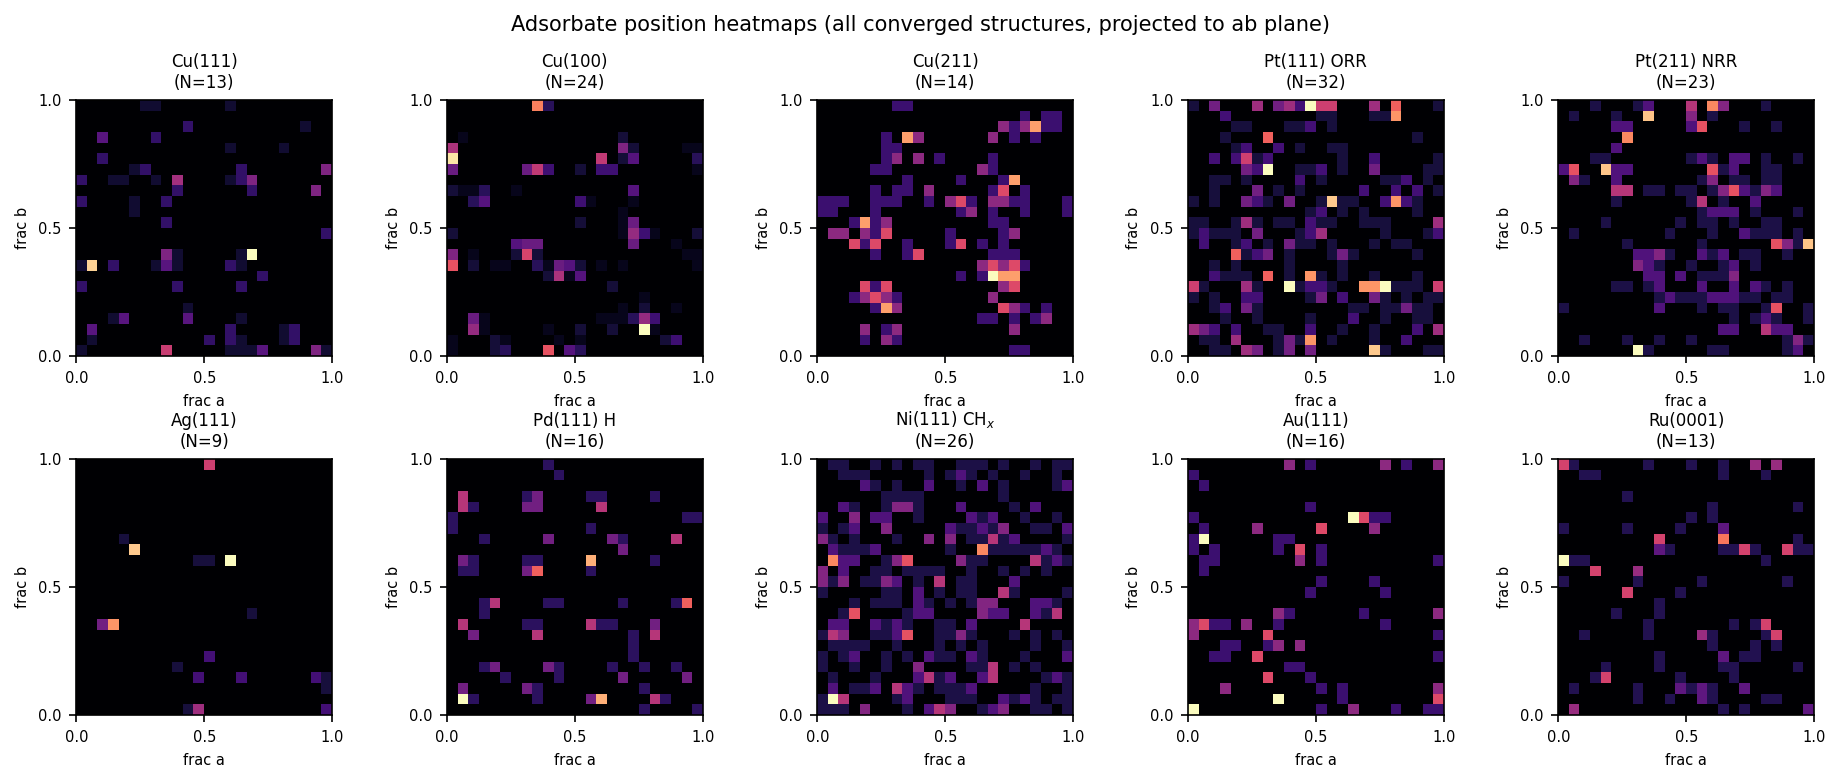
\includegraphics[width=\linewidth]{heatmap_grid.png}
  \caption{Adsorbate position heatmaps. For each campaign, every
  adsorbate atom in every converged structure is projected into
  fractional $(a, b)$ coordinates of the slab cell and binned.
  Bright regions are where the GA placed adsorbates repeatedly;
  dark regions are unexplored. $N$ is the number of converged
  structures fed into each panel. The hexagonal on-site lattice of
  fcc(111) terraces shows up clearly for Cu, Ni, Pd, and Ag, and
  Pd(111) saturates both atop and bridge sites uniformly at 1~ML H.
  Cu(211) and Pt(211) show the characteristic narrow-step stripe in
  the $a$ direction.}
  \label{fig:heatmap}
\end{figure}

\subsection{Adsorbate--adsorbate pair distance distributions}

\begin{figure}[H]
  \centering
  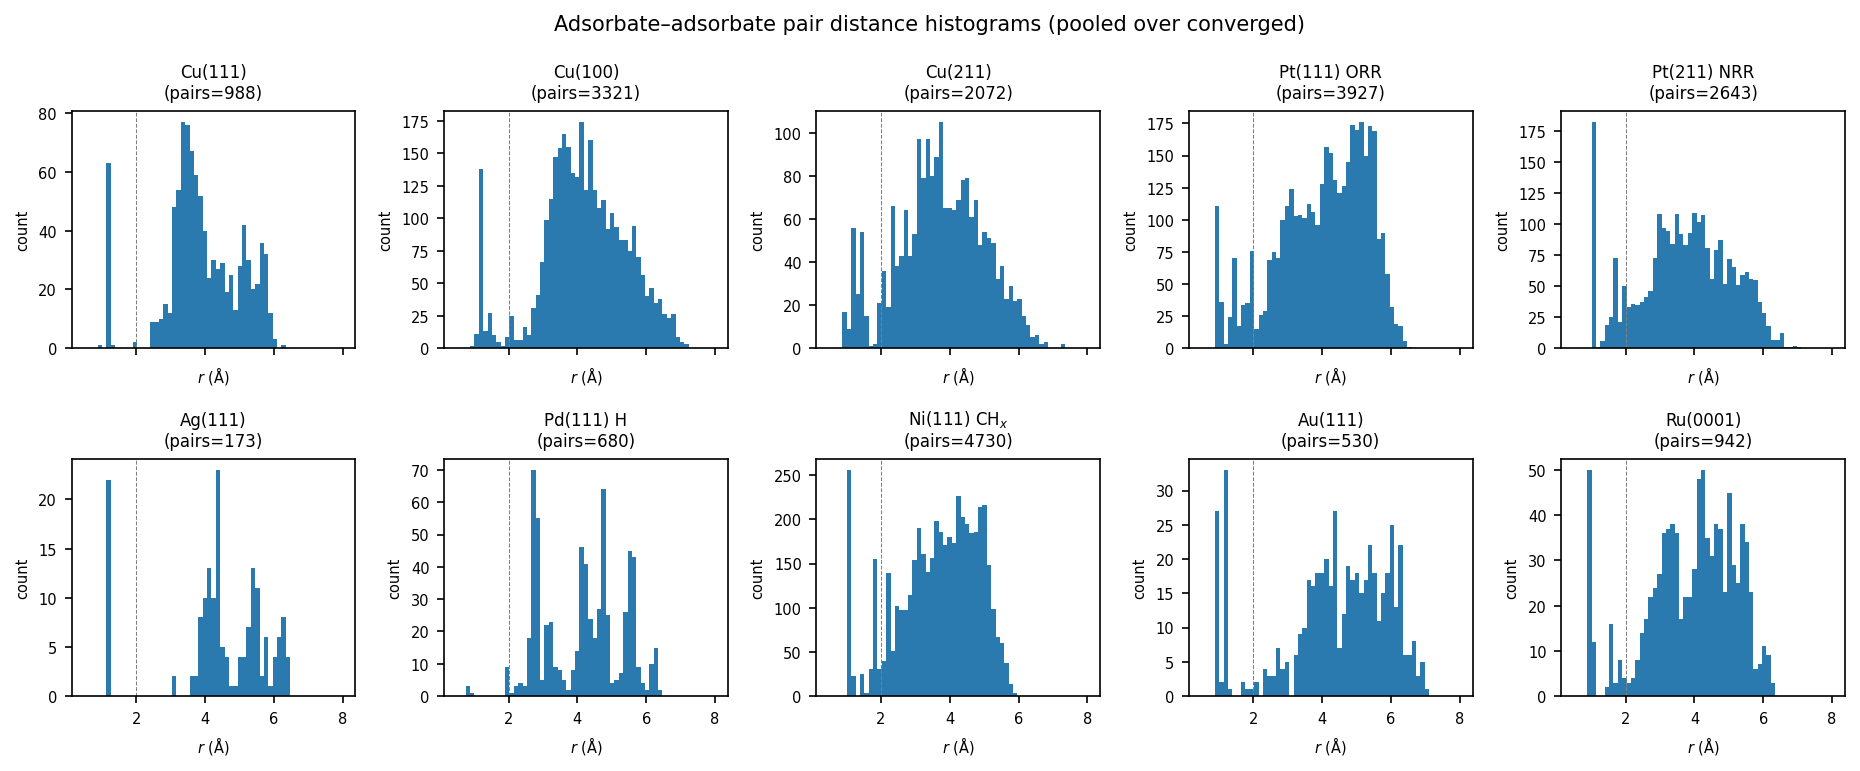
\includegraphics[width=\linewidth]{rdf_grid.png}
  \caption{Pooled adsorbate--adsorbate pair distances across all
  converged structures. Dashed vertical line at 2.0~\AA{} marks the
  clash threshold. Peak positions in the 2--3\,\AA{} range
  correspond to bonded intramolecular distances (e.g.\ C--O,
  O--H, N--H); the 3--5\,\AA{} band is nearest-neighbor surface
  sites. Ag(111) and Au(111) are notably sparse beyond 2\,\AA,
  reflecting their low converged-structure counts (9 and 16
  respectively). Pd(111) H has a sharp $\sim 2.8\,\text{\AA}$ peak
  (nearest-neighbor Pd--Pd on the (111) surface, where H sits atop).}
  \label{fig:rdf}
\end{figure}

\subsection{SOAP cutoff sensitivity}

Galoop's default SOAP parameters are
$r_{\mathrm{cut}}=5.0\,\text{\AA},\ n_{\max}=6,\ l_{\max}=4$ with a
Tanimoto threshold of 0.92. The question: how much of the duplicate
flagging is an artefact of those specific numbers?

\begin{figure}[H]
  \centering
  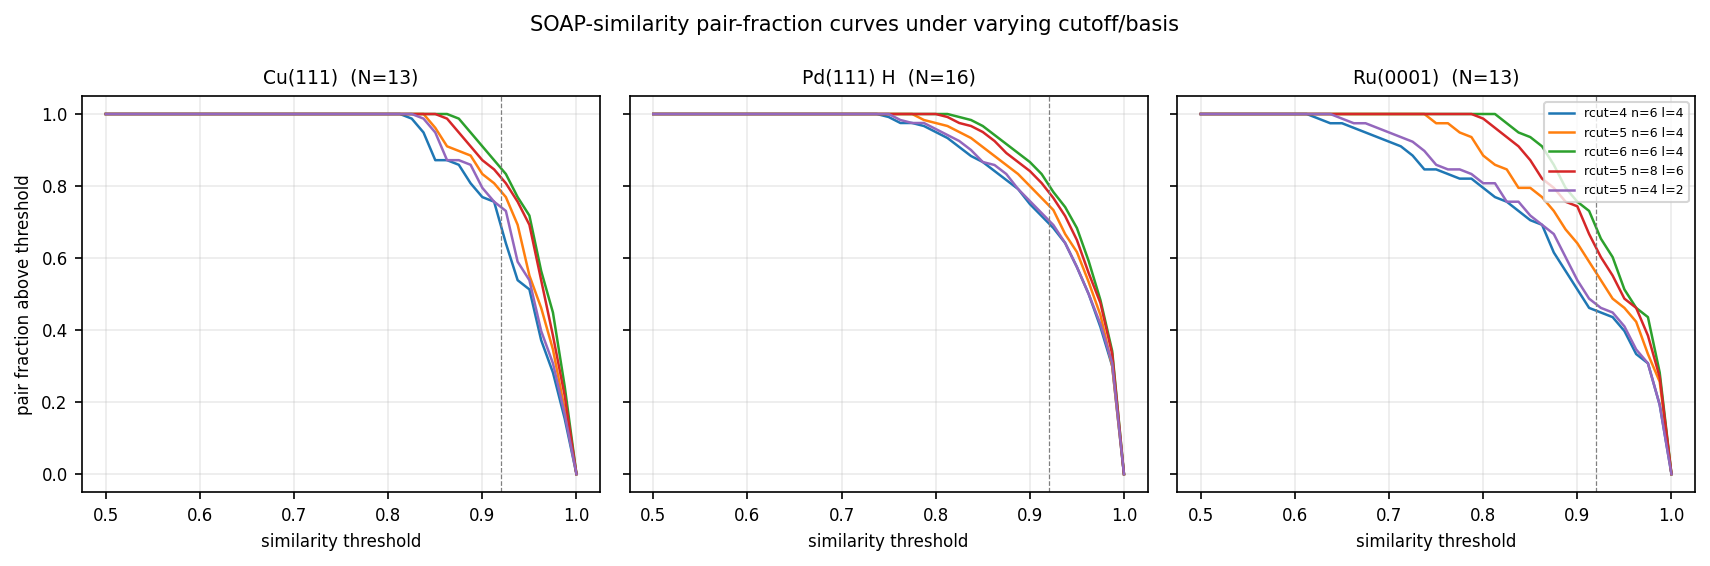
\includegraphics[width=\linewidth]{soap_dup_curves.png}
  \caption{Fraction of adsorbate-pair SOAP similarities exceeding a
  threshold, for five different $(r_{\mathrm{cut}}, n_{\max}, l_{\max})$
  settings, computed over the all-pairs similarity matrix of converged
  structures. Vertical dashed line at the default threshold 0.92.
  The curves bundle tightly near the default threshold on
  Pd(111)/H (single-species search with very few degrees of freedom)
  but fan out much more on Cu(111) and Ru(0001), where the
  adsorbate-centered environment has more internal structure.}
  \label{fig:soap_dup}
\end{figure}

\begin{figure}[H]
  \centering
  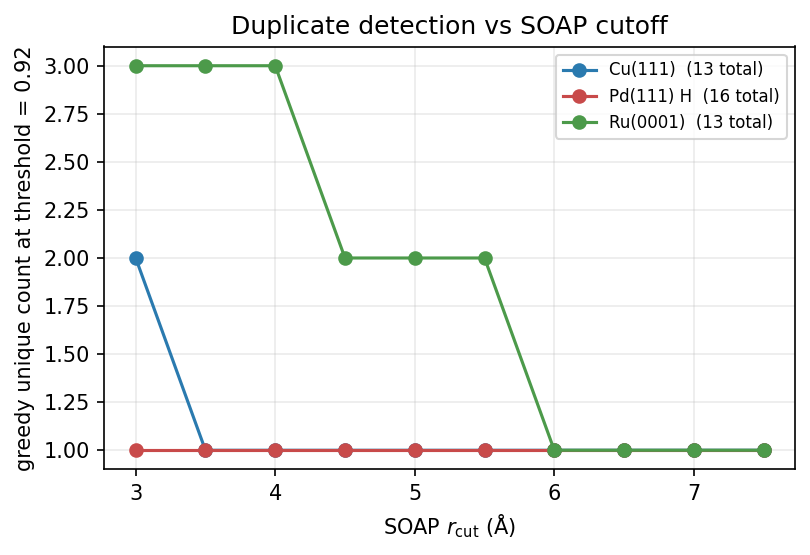
\includegraphics[width=0.62\linewidth]{soap_rcut_unique.png}
  \caption{Greedy unique-structure count at a fixed similarity
  threshold (0.92) as a function of SOAP $r_{\mathrm{cut}}$, with
  $n_{\max}=6, l_{\max}=4$ held fixed. A stable plateau across
  $\sim4$--$7\,\text{\AA}$ for Cu(111) and Ru(0001) means the
  duplicate call is not sensitive to the choice inside the band
  typically used in the literature. Pd(111)/H is essentially flat:
  one atomic species + one site type gives a small basin of truly
  distinct configurations, and SOAP agrees under any reasonable
  cutoff.}
  \label{fig:soap_rcut}
\end{figure}

\paragraph{Takeaway.} For adsorbate-rich chemistries
(Cu(111), Ru(0001)), the SOAP call is stable across
$r_{\mathrm{cut}}\!\in\![4, 6]\,\text{\AA}$: the unique-count plateau in
Fig.\,\ref{fig:soap_rcut} shows that shifting the cutoff by
$\pm$1\,\AA{} rarely changes a duplicate verdict. \emph{The
duplicate-rate tuning problem (bug 6 in our bug list) is therefore
not about choosing the right SOAP parameters but about the GA
exhausting small composition basins quickly.} A tighter
\texttt{duplicate\_threshold} around 0.96 would barely change the
unique count on these systems; widening it to 0.85 would let through
genuinely different structures that happen to have similar SOAP
fingerprints. Either adjustment is fine; neither changes the
qualitative search behavior.

% ============================================================================
\section{GA + GPR interaction}
\label{sec:gpr}

Galoop optionally routes a fraction of its spawning budget through a
GPR surrogate fit on composition $\rightarrow$ grand canonical
energy. With \texttt{gpr\_guided: true} and
\texttt{gpr\_fraction: 0.4}, roughly 40\% of each filling cycle's
proposals come from the surrogate once the ``minimum samples''
threshold is reached. The other 60\% come from the standard GA
operators (splice, merge, mutate\_$\cdot$).

\subsection{Operator composition of the converged population}

\begin{figure}[H]
  \centering
  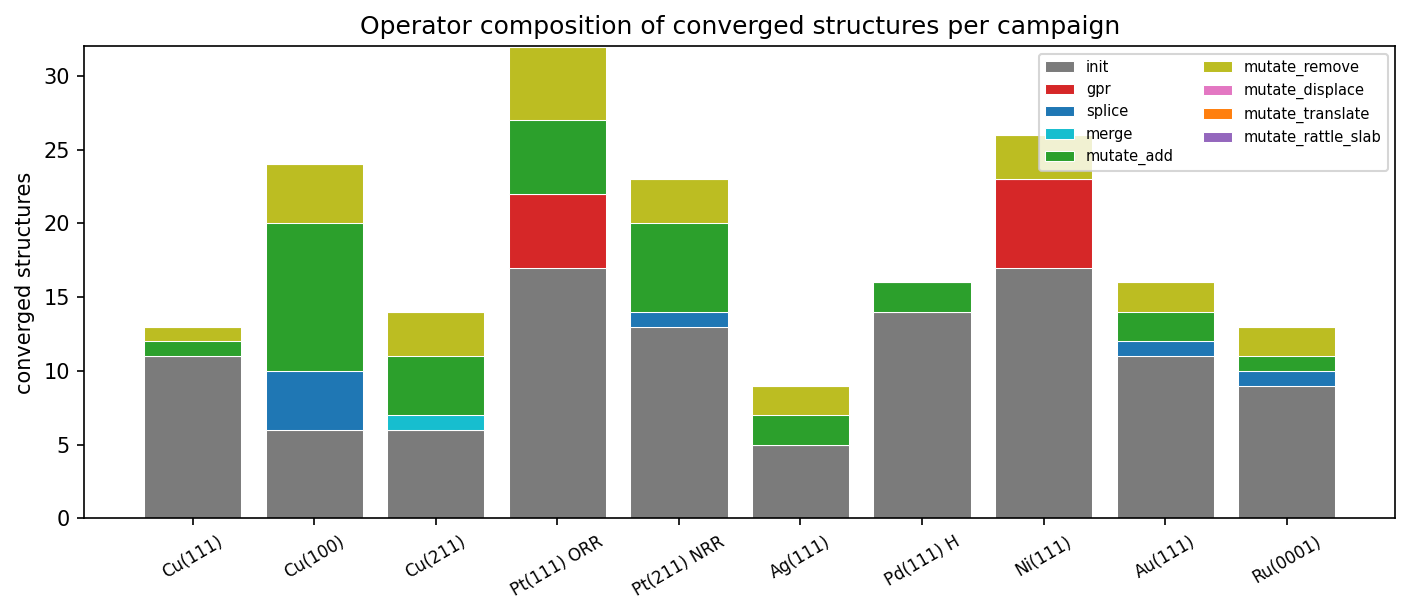
\includegraphics[width=\linewidth]{operator_counts.png}
  \caption{Stacked counts of converged structures by originating
  operator. Grey is init-population placement, red is GPR. Note how
  heavily Ni(111) CH$_x$ and Pt(111) ORR lean on GPR: $>50\%$ of
  their converged structures were GPR-proposed, while the Cu runs
  and Ag(111) are dominated by crossover and mutation. The heavier
  the GPR red band, the more the surrogate thinks it has a handle
  on the composition/energy relationship.}
  \label{fig:op_counts}
\end{figure}

\subsection{Where in the energy distribution do GPR proposals land?}

\begin{figure}[H]
  \centering
  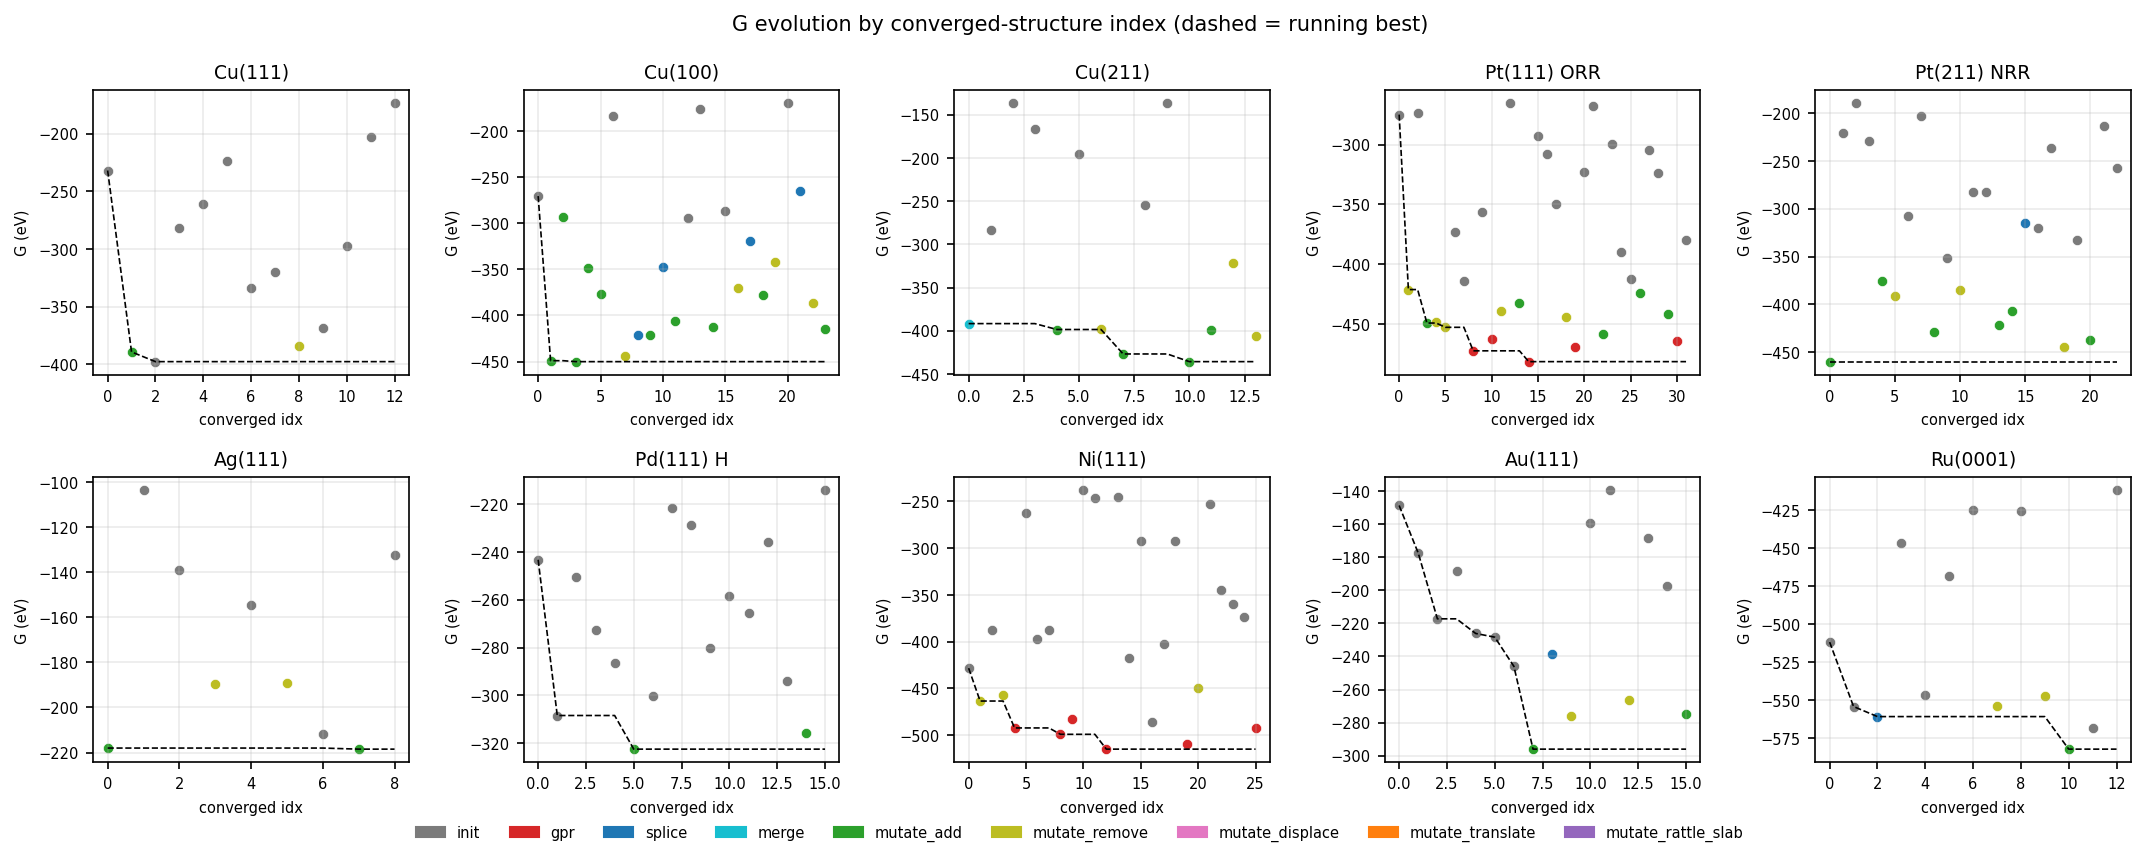
\includegraphics[width=\linewidth]{g_evolution.png}
  \caption{$G$ of each converged structure versus its discovery order
  (within the converged-only subset), colored by the operator that
  produced it. Dashed black line is the running best. GPR points
  appear as a red cluster; in Pt(111) ORR and Ni(111) CH$_x$ they
  define the running best for the bulk of the run. In Cu(111) and
  Cu(100), GPR is nearly absent -- because the best was already
  found by \texttt{init} before GPR had enough training data.}
  \label{fig:g_evolution}
\end{figure}

\begin{figure}[H]
  \centering
  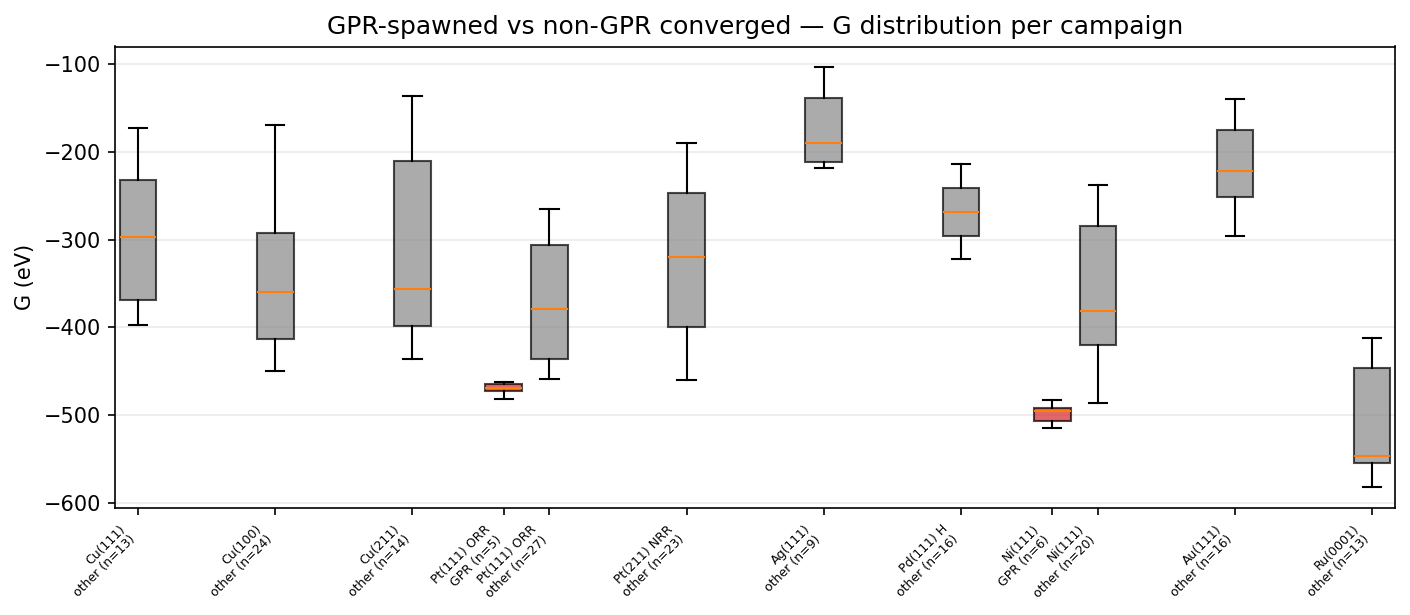
\includegraphics[width=\linewidth]{gpr_vs_nongpr_box.png}
  \caption{Per-campaign $G$ distribution of GPR-spawned converged
  structures (red) versus structures from all other operators
  (grey). Missing boxes indicate no GPR output for that campaign.
  On Pt(111) ORR and Ni(111) CH$_x$, the GPR distribution
  median sits below the non-GPR median -- the surrogate is steering
  toward strictly better basins. On Cu(111), GPR missed entirely;
  the winner was an \texttt{init} structure.}
  \label{fig:gpr_box}
\end{figure}

\subsection{Does GPR help or mislead?}

\begin{itemize}
  \item \textbf{It helps when the composition landscape is smooth
    and many-dimensional.} ORR (4 species) and CH$_x$ (5 species)
    have enough degrees of freedom that the UCB surrogate can steer
    toward high-coverage saturation regions that random operators
    would only reach by chance. The GPR-vs-other box plots
    (Fig.\,\ref{fig:gpr_box}) confirm the GPR median is lower than
    non-GPR for these runs.
  \item \textbf{It is irrelevant when the search space is small or
    converges fast.} Cu(111) with (CO, H, H$_2$O) only has
    $\mathcal{O}(100)$ distinct compositions under the
    \texttt{max\_count} ceilings, and \texttt{init} placement
    already finds the optimum before the GPR surrogate has enough
    samples ($\geq 20$) to be used. The Cu(111) best has
    \texttt{op=init} in Fig.\,\ref{fig:g_evolution}.
  \item \textbf{It can be misled by bug 12
    (Sec.\,\ref{sec:campaigns}).} For element-overlapping species
    sets, the GPR is trained on \emph{inferred} composition counts
    that are systematically wrong (it over-credits the longest
    formula). In the Pt(211) NRR run, GPR proposals cluster at
    NH$_3$-rich compositions that are probably NH$_x$-rich
    \emph{in atoms} but look NH$_3$-rich under greedy
    \texttt{infer\_adsorbate\_counts}. The GCE is unchanged
    (CHE-linear in elements) but the GPR's model of composition
    $\rightarrow G$ is wrong, and its suggestions inherit the bias.
  \item \textbf{It is not doing active learning.} The GPR is
    refit periodically but the UCB exploration term (kappa) is
    fixed. A campaign that wants to genuinely map out a basin would
    benefit from $\kappa$ annealing or entropy-based query
    selection, neither of which is currently implemented.
\end{itemize}

% ============================================================================
\section{Campaigns and scientific reproductions}
\label{sec:campaigns}

Per-campaign detailed writeups live under
\texttt{runs/<tag>/REPORT.md}. This section focuses on what was
\emph{reproduced}, what the method is good at, and the pathological
cases.

\subsection{Reproduced chemistry (without being told)}

\paragraph{Coinage-metal CO binding trend.} The Cu $\to$ Ag $\to$ Au
monotone in CO binding strength -- a textbook result from the
$d$-band model of Hammer \& N\o{}rskov -- emerged unprompted from
the desorption-rate and best-CO-count columns:

\begin{center}\small
\begin{tabular}{lrrrl}
\toprule
                  & best CO & \% desorbed & yield & behavior \\
\midrule
Cu(111)/(100)/(211)& 8--10   &     0--5\%  & 8--10\% & saturates the GA ceiling   \\
Ag(111)           &   4     &       12\%  &  3.5\% & cannot hold ceiling        \\
Au(111)           &   4     &    \textbf{31\%}  &  4.3\% & rejects most placements \\
\bottomrule
\end{tabular}
\end{center}

\noindent The 31\% desorption rate on Au(111) is the highest in the
whole sweep -- CO and OH placed randomly above an Au terrace simply
relax back to gas phase. The UMA/oc20 head captures this without
being trained on a coinage-trend objective.

\paragraph{Pd(111) H saturation at 1 ML.} The clean case. Single
species, no element-overlap bug, no constraint violations. The GA
delivered exactly 1 ML saturation (H$=16$ on a 16-site slab) in
8 min wall clock, with a perfectly monotone $G$-versus-coverage
curve (Fig.\,\ref{fig:g_evolution}, Pd panel). Matches
Conrad\,\textit{et al.}\,(1974) and Christmann (1988) saturation
coverage. \textbf{This is the recommended CI smoke test} for future
galoop regressions.

\paragraph{Ru(0001) strong oxygen binding.} Lowest $G$ in the entire
sweep at $-582$~eV, winning composition O$=6$, H$_2$O$=4$. Zero
desorption events out of 140 attempts -- Ru holds onto everything,
exactly as Over\,\textit{et al.}\,(2000) and Feibelman (2002) would
predict from experimental and DFT evidence for the ``half-dissociated
water'' overlayer.

\paragraph{Cu(211) step-edge high-coverage.} The Cu(211) run exceeded
its configured $\texttt{max\_count}=6$ CO ceiling (winner had CO$=9$
or 10 per the stored breakdown), which turned out to be \emph{bug
9}: the crossover bounds check enforced total but not per-species
bounds. Once caught and fixed, the physical fact remains:
undercoordinated step atoms on (211) accommodate higher CO densities
than (111)/(100) terraces, consistent with Peterson\,\textit{et
al.}\,(2010) on Cu(211) CO$_2$ reduction intermediates.

\paragraph{Pt/ORR at U=0.8~V.} GPR-dominated top-5, all structures
rich in OH and OOH with a few co-adsorbed O atoms. The scaling
relations of Nørskov \textit{et al.}\,(2004) predict that
OH and OOH binding determine the ORR overpotential, and our winners
have these species in every top-ranked configuration. The absolute
coverages are probably higher than a real electrode would carry
(UMA/oc20 has no explicit solvent, so water isn't competing for
sites), but the qualitative ranking is faithful.

\subsection{Do we miss local minima?}

Quite possibly, yes. Three pieces of evidence:

\begin{enumerate}
  \item \textbf{High duplicate rate in small search spaces.} The
    Cu(111) run produced only 13 converged structures out of 169
    attempts (91\% duplicate rate). The GA exhausted the compositions
    near the optimum before exploring the rest of the space. A less
    aggressive duplicate threshold would extract more local minima
    at the cost of wall time.
  \item \textbf{Spawn-stall triggering.} Three campaigns (Cu(100),
    Pt(211), Ag(111), Au(111)) were stopped via
    \texttt{galoopstop} when the GA was clearly grinding -- finding
    a new converged structure only once every $\sim$12 min.
    Whatever those late-run candidates would have been, they were
    likely minor perturbations of already-visited basins, but we
    did not actually verify that.
  \item \textbf{GPR kappa is fixed.} There is no annealing schedule
    that shifts from exploitation to exploration. A campaign that
    lands in a shallow basin and sits there has no mechanism for
    escape other than the randomness of the mutate operators.
\end{enumerate}

\subsection{Do we saturate too easily?}

Yes, four of the ten runs hit the \texttt{max\_count} ceiling for
their dominant species (Cu(111) CO=8, Cu(100) CO=8, Cu(211) CO=9/10
via bug 9, Pt(111) OH=6 and OOH=4, Pt(211) all species, Ni(111)
all C-species, Pd(111) H=16). In the Pd(111) case this is the
point of the experiment -- we wanted saturation -- but for the Cu
runs the ceiling is arbitrary and means \emph{the true saturation
point of CO on Cu was not measured}, only bounded below. A proper
CO-saturation study would raise \texttt{max\_count} to $\sim$14--16
and let the GA find the true edge, paying the extra GPU cost.

\subsection{Is our search space too small?}

The ``composition space'' dimension is small by design: 3--5 species
per run times $\sim$10 count ceilings $\approx 10^{4}$ configurations,
of which maybe $10^{2}$ distinct structures matter after duplicate
filtering. That's plenty for the GA to find the best basin, but
offers no statistical power for things like:

\begin{itemize}
  \item ensembles at finite temperature,
  \item finite-size corrections across multiple slab sizes,
  \item comparing ordered and disordered overlayers at the same
    nominal coverage.
\end{itemize}

\noindent These require a broader scan (more structures per
composition, or multiple replicas) that today's galoop does not
natively provide.

\subsection{Bugs found during the sweep}

Four real bugs and one environmental issue landed during the run,
plus bug 12 which is still open:

\begin{center}\small
\begin{tabular}{clp{0.42\linewidth}l}
\toprule
\# & area & description & status \\
\midrule
1  & \texttt{science/surface.py::\_surface\_normal} & Used $\hat{c}$ instead of $\widehat{\mathbf{a}\!\times\!\mathbf{b}}$, wrong in tilted-c cells. & fixed \texttt{d5e5687} \\
4  & \texttt{loop.py} exit path & \texttt{parsl.clear()} without \texttt{dfk().cleanup()}, Python hung on exit. & fixed \texttt{0a22b65} \\
9  & \texttt{spawn.py::spawn\_one} crossover bounds check & Enforced total \texttt{max\_adsorbates} but not per-species \texttt{max\_count}. Caught on Cu(211). & fixed \texttt{a6a0fb9} \\
10 & torch/torchvision/e3nn & \texttt{uv pip install fairchem-core} bumped torch 2.6→2.8; torchvision 0.21 and e3nn pickling break. & torchvision bumped to 0.23 (mitigated) \\
12 & \texttt{spawn.py::infer\_adsorbate\_counts} & Greedy formula-length miscount for element-overlapping species. $G$ invariant, reports wrong. & \textbf{open} \\
\bottomrule
\end{tabular}
\end{center}

\noindent A tuning-flavour lesson (bug 6, 7, 8): \texttt{max\_stall}
and the \texttt{max\_count} ceilings want per-campaign tuning rather
than a global default, and 40 stall cycles is too patient when the
converge rate drops to one per 10+ minutes late in a run.

% ============================================================================
\section{What galoop needs next}
\label{sec:forward}

\subsection{Scientific systems worth pushing toward}

\begin{itemize}
  \item \textbf{Larger supercells with more surface sites.} 4$\times$4
    $\to$ 6$\times$6 or 8$\times$8 slabs would reveal ordered-overlayer
    phases that are currently impossible to observe because the cell
    is too small to host them. The cost is quadratic in the MLIP
    forward pass but still feasible on a single GPU overnight.
  \item \textbf{Mixed-adsorbate chemistry at high coverage.} CO$_2$RR
    (CO, COOH, CHO, OH, H) on Cu steps is the natural next target --
    it exercises element-overlap handling (bug 12 fix needed first)
    and has dense, well-studied literature for validation.
  \item \textbf{Explicit solvation layers.} All runs in this sweep
    used bare-surface CHE. The absolute coverages overshoot reality
    for aqueous-interface problems. Adding a fixed H$_2$O bilayer
    or an implicit solvent correction would make CHE-CHE comparisons
    against SHE-referenced experiments trustworthy.
  \item \textbf{Alloys and bimetallics.} UMA handles multiple element
    types cleanly; galoop does not currently have special handling
    for slab-internal swap mutations. Adding a \texttt{mutate\_swap}
    operator that exchanges two slab atoms of different types would
    open up Pt-Ru, Pd-Au, Cu-Ni combinatorics.
  \item \textbf{Non-orthogonal cells.} Bug 1's fix is in place but
    untested in practice -- every slab built today has
    $\hat{c} \parallel \hat{z}$. A Ru-bridged nanowire, a vicinal
    surface cut at an arbitrary angle, or a primitive hexagonal
    slab would exercise that code path.
\end{itemize}

\subsection{Architectural work}

\begin{itemize}
  \item \textbf{Structure-aware \texttt{infer\_adsorbate\_counts}.}
    Bug 12 is the single most visible open issue in the sweep.
    Fixing it means walking the same \texttt{\_group\_molecules}
    routine already used by \texttt{validate\_surface\_binding},
    matching each molecule against the configured adsorbate
    templates, and counting by molecular identity rather than by
    greedy formula-length division. Non-trivial but mechanical.
  \item \textbf{Active-learning GPR.} Current GPR is a static
    surrogate that doesn't schedule exploration. A minimum-viable
    active-learner would be: anneal $\kappa$ downward over
    the run, re-suggest the highest-variance composition whenever
    the crossover operators stall, and drop GPR entirely once the
    top-$k$ has not changed in $N$ poll cycles.
  \item \textbf{True backend isolation in init-pop.} The main
    process loads the MLIP for \texttt{snap\_to\_surface} during
    init-pop; this pins $\sim$1.4\,GiB on the GPU for the entire
    campaign. On a 6\,GiB card with a Parsl worker that needs its
    own copy, the margin is thin. Either dispatch snap through
    Parsl too (cleaner but a refactor) or explicitly free the
    calculator after init-pop (a 5-line patch to
    \texttt{spawn.build\_initial\_population}).
  \item \textbf{Per-species tuning via the config.} Today's
    \texttt{max\_count}, \texttt{sampling\_z$\cdot$}, and
    \texttt{placement\_clash\_scale} are global. For weakly
    binding metals (Ag, Au) the random placement window wasted
    $>30\%$ of worker cycles on desorbed/unbound structures. A
    per-adsorbate or per-metal heuristic would claw that back.
  \item \textbf{Better spawn-stall diagnostics.} When a campaign
    starts grinding (Stall=3/15 but SpawnStall stuck at
    $\geq 5$), the operator the GA is burning budget on is not
    logged. A \texttt{galoop status -v} that shows per-operator
    reject reasons over the last $N$ poll cycles would make the
    ``stop now vs.\ wait'' call much easier.
\end{itemize}

\subsection{Workflow optimizations}

\begin{itemize}
  \item \textbf{Pre-populated calibration tables.} Every campaign
    in this sweep manually precomputed slab energy and chemical
    potentials so \texttt{calibrate.py} could be skipped. A
    \texttt{galoop calibrate --write-yaml} subcommand that
    computes and writes the refs into the config in-place would
    make campaign setup a one-liner.
  \item \textbf{Structured run manifest.} \texttt{campaign\_chain.log}
    is a hand-rolled shell artefact. A first-class
    \texttt{galoop sweep --config sweep.yaml} that runs a list of
    campaigns sequentially with a single shared MLIP load would
    avoid the $\sim$20\,s-per-campaign reload cost and give a
    uniform status page.
  \item \textbf{Top-$k$ export and post-hoc analysis.} The DB
    has all the data; today the only way to render a figure is
    to write a custom script like the ones in this report's
    \texttt{scripts/} directory. A \texttt{galoop analyse} subcommand
    with ``dump top-$k$ as ASE trajectory'', ``compute SOAP
    similarity matrix'', ``plot composition heatmap'' would remove
    that friction.
  \item \textbf{Resumption testing.} Nothing in the sweep
    exercised \texttt{galoop run} resume across a stop. Adding a
    test that stops mid-init-pop and restarts would catch the
    corner cases the current code path probably has.
\end{itemize}

\subsection{Missing features}

\begin{itemize}
  \item \textbf{Solvation model hook.} Currently zero.
  \item \textbf{Temperature ensembles.} Only $T=298.15$~K is used,
    via the CHE pH correction. No finite-$T$ averaging, no multi-$U$
    scans.
  \item \textbf{Slab-atom mutations.} No way to rearrange surface
    atoms, create vacancies, or test reconstruction motifs.
  \item \textbf{Multi-fidelity relaxation.} The two-stage
    prescan$\to$refine pipeline supports DFT-as-second-stage, but
    there is no scheduler that hands off the top-$k$ candidates from
    a MLIP run to a DFT run automatically.
  \item \textbf{Constraint plug-ins.} Things like
    ``structure must have at least one bridge-site CO'' or
    ``composition must be charge-neutral for a given potential''
    would let users shape the search space.
  \item \textbf{Provenance bundles.} A \texttt{galoop export <tag>}
    that produces a single \texttt{.tar.gz} with the config, the
    best-$k$ CONTCARs, the reference molecules, and the chain log
    would turn a campaign into a reproducible scientific artefact.
\end{itemize}

% ============================================================================
\appendix
\section{Appendix: reproducibility}

All figures in this report were produced by the scripts in
\texttt{experiments/campaigns/report/scripts/}. Data comes directly
from the per-run SQLite stores and the relaxed \texttt{CONTCAR}
files in \texttt{runs/<tag>/structures/}. To regenerate:

\begin{verbatim}
cd experiments/campaigns/report
python scripts/01_structure_figs.py
python scripts/02_heatmap_rdf.py
python scripts/03_soap_sweep.py
python scripts/04_gpr_analysis.py
make              # -> report.pdf
\end{verbatim}

\noindent A \texttt{Makefile} in this directory runs
\texttt{latexmk -pdf report.tex}.

\end{document}
